\documentclass{article}
\usepackage{graphicx}
\usepackage{geometry}
\usepackage{listings}
\usepackage{hyperref}
\usepackage[italian]{babel}

\usepackage{subcaption} % for subfigures

\geometry{
	a4paper,
	top = 2cm,
	bottom = 2cm,
	left = 2cm,
	right= 2cm,
}

\begin{document}
\section{Introduzione ed obiettivi}
Il seguente documento riporta i passi logici seguiti e le informazioni raccolte per quanto riguarda l'analisi del file eseguibile \textbf{hw3.exe}. Il file è stato analizzato mediante l'uso dei seguenti tools 
\begin{itemize}
\item disassemblatore Ghidra
\item debugger OllyDbg
\end{itemize}
L'obiettivo dell'analisi è quello di \textbf{trovare il codice di sblocco che rende funzionante l'applicazione}, nel rapporto vengono riassunti i passi logico-deduttivi fatti e le informazioni raccolte durante le attività di reverse code engineering.\\La stesura del documento utilizza varie assunzioni che derivano dalla precedente analisi dell'eseguibile \textbf{hw2.exe}, in quanto questo presenta diverse analogie con il file \textbf{hw3.exe}.
\section{Raccolta informazioni generali sul file}
In una prima fase, sono state ricostruite tutte le informazioni che erano già state trovare durante l'analisi del file \textbf{hw2.exe}, comunque necessarie per ricostruire il funzionamento generale del programma. Anche in questo caso, lanciando il file eseguibile, compare una finestra che permette di impostare un timeout per lo spegnimento della macchina host. Se però non si fornirà il codice corretto che rende funzionale l'applicativo, lo spegnimento effettivo della macchina non avverrà. Sono quindi stati analizzati i blocchi fondamentali del programma e tutte le informazioni trovate, come ad esempio l'associazione dei nomi delle funzioni inserite in Ghidra, sono stati riportati anche in OllyDbg, mettendo le label sui corrispettivi indirizzi di memoria.
\subsection{Ricerca del WinMain}
La ricerca del \texttt{WinMain}, che è il punto d'ingresso per le applicazioni Windows basate su GUI, è avvenuta mediante Ghidra individuando il blocco di codice in cui è presente il \textbf{Messsage Loop}.\\Consultando le funzioni importate dalla DLL \texttt{User32}, sono state trovate le API 
\begin{itemize}
\item \texttt{GetMessageA}
\item \texttt{TranslateMessage}
\item \texttt{DispatchMessageA}
\end{itemize}
e consultando i riferimenti a tali API si vede che queste vengono chiamate una sola volta, nella funzione \texttt{FUN\_004024e0} e quindi tale funzione è la \texttt{WinMain}.
\subsubsection{Analisi del file mapping}
La prima funzione chiamata all'interno della \texttt{WinMain} è la \texttt{FUN\_00401560}. Tale funzione è stata analizzata avvalendosi del tool di de-compilazione di Ghidra:
\begin{itemize}
	\item la prima funzione chiamata è la API \texttt{GetModuleFileNameA}, a cui viene passato come primo parametro il valore \texttt{NULL}. Questo ha l'effetto di recuperare il full path del file eseguibile del processo corrente
	\item viene poi invocata la \texttt{CreateFileA}, una API usata per creare o accedere in I/O un file. In questo caso, dati i parametri che vengono passati in input, si richiede di aprire il file in lettura solo se questo esiste già
	\item la \texttt{GetModuleFileNameA} in caso di successo, restituisce un handle al file. Se tale handle è valido, segue la chiamata alla API \texttt{GetFileInformationByHandle}. Tale API permette di recuperare le informazioni legate ad un file, che vengono restituite nel secondo parametro, di tipo struttura \texttt{LPBY\_HANDLE\_FILE\_INFORMATION}
\end{itemize}
A questo punto, viene salvata la parte bassa della taglia del file nella variabile globale \texttt{DAT\_004070e8} che è stata rinominata come \texttt{low\_file\_size}, per poi proseguire con altre 2 chiamate ad API:
\begin{itemize}
	\item prima, viene invocata la \texttt{CreateFileMappingA}, che crea o apre un oggetto file mapping per un file. Il 3° parametro della funzione è \texttt{flProtect}, che specifica la protezione delle regioni di memoria del file mapping ed in questo caso i flag specificati dicono che il file corrispondente all'handle è eseguibile ed inoltre che le pagine siano mappate per accessi read-only o copy-on-write.
	\item se la funzione ha successo, viene restituito un handle al file mapping appena creato, utilizzato come primo parametro nella chiamata alla \texttt{MapViewOfFile}. L'API mappa la vista del file mapping nello spazio d'indirizzamento del processo corrente. Il secondo parametro della funzione specifica i permessi di accesso alle pagine mappate in memoria, che in questo caso viene settato con la macro \texttt{FILE\_MAP\_READ}, ovvero sono possibili solo accessi read-only.\\Il risultato di questa API è l'indirizzo iniziale della vista della file map, che viene salvata nella variabile globale \texttt{DAT\_004070e4}. Tale variabile è stata rinominata \texttt{file\_map\_startaddr}
\end{itemize}
Questa funzione è stata rinominata come \texttt{create\_file\_map}

\subsubsection{Inizializzazione della struttura dati}
Esattamente come accadeva per il file \textbf{hw2.exe}, vi è la funzione \texttt{FUN\_00401830} in cui avviene l'inizializzazione della struttura di dati che verrà usata nel programma, rinominata quindi come \texttt{app\_ds}. Infatti, all'interno di tale funzione, vi è l'inizializzazione:
\begin{itemize}
\item del valore del timeout corrente, inizializzato a 0, ad offset 0 della struttura dati
\item della lunghezza del tick, inizializzato a 1000, ad offset 4
\item del timeout per l'applicazione, inizializzato a 1800, ad offset 12
\item dei due buffer di caratteri, uno di 128 byte ad offset 24 ed uno di 16 caratteri ad offset 152
\item del capo ad offset 20, a cui viene associato il valore del parametro passato come input dalla WinMain, ovvero la variabile globale \texttt{DAT\_004040e0}.
\end{itemize}
La struttura dati, a cui è stato assegnato il nome \texttt{app\_ds}, è stata inizialmente creata con una taglia di 192 byte, come avvenuto per il file precedente.\\Consultando le variabili globali nel .bss, è possibile notare che le due variabili definite in precedenza, ovvero \texttt{low\_file\_size} e \texttt{file\_map\_startaddr} si trovano esattamente sotto l'ultimo campo della struct, quindi è ragionevole supporre che tali variabili siano in realtà due campi della struttura, rispettivamente ad offset 200 e 196.
\subsubsection{Caricamento dinamico della \texttt{OutputDebugString}}
Dopo l'inizializzazione della struttura dati, vi è una chiamata alla funzione \texttt{FUN\_004016f0}. Aprendo tale funzione con Ghidra, sono presenti diversi meccanismi anti-disassembling tutti basati sull'utilizzo della sequenza di istruzioni \texttt{eb ff c0 48} che realizza uno dei modi per ottenere una misura di disassembling impossibile. Per risolvere il problema, si è proceduto come segue:
\begin{itemize}
\item si pulisce il codice disassemblato, tramite l'opzione "clear code bytes"
\item si riprende il disassemblaggio dalla prima istruzione dopo la "48", così da ottenere il corretto codice
\item si sostituisce ad ognuna delle istruzioni che compongono il codice \texttt{eb ff c0 48} con una \texttt{NOP} (codice operativo 90) per poter ottenere un codice de-compilato correttamente leggibile.
\end{itemize}
Si arriva quindi al decompilato in \ref{Fig1}.\\Consultando tale funzione, si capisce che
\begin{itemize}
\item viene scritta nella variabile automatica \texttt{local\_2d}, rinominata \texttt{local\_str} la stringa "kernel32.dll"
\item chiamata la \texttt{LoadLibraryA}, quindi caricata la libreria \texttt{kernel32.dll} dinamicamente
\item viene poi messa nello stesso array di prima la stringa "OutputDebugStringA"
\item viene infine chiamata la \texttt{GetProcAddress}: questa API restituisce l'indirizzo della funzione \texttt{OutputDebugString}
\end{itemize}
Tale risultato viene salvato nella variabile globale \texttt{DAT\_004070ec}, anche in questo caso la variabile è stata inclusa come campo della struttura dati, ad offset 204.
\subsection{Analisi della \texttt{WinProc}}
È stata poi definita la \texttt{WinProc}, ad indirizzo 00401de0. Aprendo la funzione ed avvalendosi del tool di de-compilazione di Ghidra, è possibile vedere in prima analisi che la struttura del codice è molto simile a quella del file \textbf{hw2.exe}: i messaggi gestiti sono sempre i soliti, relativi alle varie fasi che compongono il ciclo di vita di un'applicazione basata su finestra per Windows:
\begin{itemize}
\item \texttt{WM\_CREATE}, con codice 1;
\item \texttt{WM\_DESTROY}, con codice 2;
\item \texttt{WM\_SIZE}, con codice 5;
\item \texttt{WM\_PAINT}, con codice 15;
\item \texttt{WM\_COMMAND}, con codice 273
\end{itemize}
Ad esempio, all'interno del blocco della \texttt{WM\_CREATE} vengono inizializzati tutti gli handles delle finestre e del bottone che compongono l'applicazione, per inserirli all'interno di un array nella struttura dati, ad offset 168.\\Sono stati quindi ricostruiti tutti i campi mancanti della struttura dati, riassunti in \ref{Fig2}
\section{Risoluzione delle misure anti-debugging}
Una volta ricostruite le informazioni fondamentali per il programma all'interno di Ghidra, queste sono state riportate su OllyDbg ed è stato utilizzato questo tool per riuscire a trovare il codice di sblocco. Il primo problema che è stato affrontato riguarda la presenza di una o più tecniche anti-debugging presenti all'interno del codice: difatti, se si tenta di aprire il programma mediante OllyDbg e si lancia la sua esecuzione (f9), ci si aspetterebbe che venga mostrata la finestra per inserire il timeout e premere il bottone che lo faccia partire. Ma in realtà, non appena si lancia, il debugger termina la sua esecuzione.
\subsection{Patching per la \texttt{IsDebuggerPresent}}
Fra le funzioni chiamate nel WinMain, è possibile individuare la \texttt{FUN\_004024a0}, al cui interno vi è la chiamata alla API \textbf{\texttt{IsDebuggerPresent}}:
\begin{itemize}
\item si valuta il risultato di ritorno di tale API e se è pari a 0, si termina l'applicazione
\item se invece il valore è diverso da 0, si chiama l'API \texttt{ShowWindow} e si ritorna al WinMain
\end{itemize}
Siccome l'applicazione viene eseguita all'interno del debugger, il valore di ritorno sarà sempre 0, quindi per risolvere tale problema in OllyDbg è stata applicata una patch modificando alcune delle istruzioni del codice Assembly, come viene mostrato in \ref{Fig3}.\\A questo punto, è stato possibile analizzare tutta la struttura del programma mediante l'utilizzo di OllyDbg: se si fa "run" tramite debugger, anche in questo caso l'esecuzione rimane running ma senza mostrare la finestra mentre ci si aspetterebbe di vederla comparire.
\subsection{Accesso alla PEB}
L'analisi si è spostata sulla WinProc, per verificare se ci fosse qualche altro meccanismo anti-debugging. La scelta è stata quella di analizzare la WinProc in quanto prima di mostrare la finestra, verranno sicuramente gestiti alcuni messaggi dalla procedura, per creare la finestra ed inserivi gli elementi all'interno.\\È stato messo un breakpoint sulla prima istruzione della WinProc, per poi procedere con l'analisi step-by-step dopo aver rilanciato il programma. La prima funzione che si trova all'interno del codice è la \texttt{FUN\_00401dc0} a cui viene passato come parametro il codice del messaggio ricevuto. Analizzando la funzione, sia con Ghidra che con OllyDbg, è possibile capire che
\begin{itemize}
\item viene acceduto il segmento FS ad offset 0x30. Tale offset contiene la struttura dati PEB
\item all'offset 0x2 della PEB c'è un campo \texttt{BeingDebugged}, pari a 0 se è presente un debugger
\end{itemize}
Il risultato della funzione è quindi quello di incrementare il valore del codice del messaggio di uno: l'effetto di tale funzione è quindi di impedire a ciascun messaggio per cui vi è una gestione esplicita, come la creazione della finestra o il paint della stessa, di venire correttamente gestito, in quanto il valore verrebbe sempre incrementato di 1, andando a finire sulla gestione di default.\\Quindi è stata applicata una patch in OllyDbg che andasse a mascherare tale chiamata a funzione mediante una serie di NOP, come mostrato in \ref{Fig4}.\\A questo punto, se si apre il nuovo file patchato e si prova a far partire il programma, viene mostrata la finestra, ma senza contenuto e dopo qualche secondo il debugger crasha. Se si prova ad aprire il programma normalmente, quindi fuori da un debugger, viene mostrato il message box riassunta in \ref{Fig5}.\\In ogni caso, una volta risolto questo problema, sono stati messi dei breakpoint su ognuna delle prime istruzioni dei blocchi di codice per la gestione dei messaggi nella WinProc, in modo da poter analizzare singolarmente la gestione di ogni messaggio. 
\subsection{Path per la \texttt{OutputDebugString}}
Precedentemente, era stato caricato in una variabile globale l'indirizzo della API \texttt{OutputDebugString}, quindi ci si aspetta che tale funzione venga richiamata in qualche altro punto del codice.\\Tornando sempre ai breakpoints nella \texttt{WinProc}, è stato analizzato il blocco di codice per la gestione del comando \texttt{WM\_PIANT} (codice 5): dopo aver chiamato le diverse API per ridisegnare la finestra, vi è una CALL alla funzione \texttt{FUN\_00404000}:
\begin{itemize}
\item dentro OllyDbg, è stato messo un breakpoint alla prima istruzione di tale funzione
\item una volta che l'esecuzione arriva al breakpoint, proseguendo con "step over", si arriva al punto in cui viene caricato sullo stack la stringa "\%s\%s\%s\%s\%s\%s\%s\%s\%s\%s\%s\%s\%s\%s\%s\%s"
\item viene poi preparata la CALL alla funzione \texttt{OuputDebugString}
\end{itemize}
La \texttt{OuputDebugString} è una funzione che permette di inviare una stringa al debugger, utilizzando una formattazione "printf-like", quindi la stringa di formato costituita dai 16 "\%s" avrà l'effetto di dire al debugger di dover andare a leggere 16 parametri dallo stack, questo porterà ad accedere ad un indirizzo di memoria invalido, mandando quindi in crash il debugger stesso, in quanto verrà generato un segmentation fault.\\Per risolvere è stata applicata una patch, andando a mettere una serie di NOP al posto della CALL alla funzione \texttt{FUN\_00404000}.\\
\subsection{Risoluzione del Message Box "Internal Error"}
\subsubsection{Manipolazione del file mapping}
All'interno del blocco di codice che gestisce il messaggio \texttt{WM\_CREATE}, dopo aver creato tutti gli handles alle finestre, aver inizializzato il timeout ed aver registrato tale timeout chiamando la \texttt{SetTimer}, vi è un'ultima CALL alla funzione \texttt{FUN\_004016b0}. In tale funzione, si accedono le due variabili globali inizializzate precedentemente nella \texttt{init\_ds} della \texttt{WinMain}, ovvero \texttt{file\_map\_startaddr} e \texttt{low\_file\_size}. Arrivando con un breakpoint in OllyDbg alla prima istruzione di tale funzione, è stato possibile analizzarne il contenuto:
\begin{itemize}
\item La funzione accede al campo ad offset 192 della struttura dati, impostandolo a 0
\item il registro EAX contiene la taglia del file, che viene divisa per 4 mediante uno shift a desta e viene sottratta di 256
\item EDX contiene l'indirizzo iniziale del file mapping, a cui viene aggiunto il valore 400
\item all'interno di un ciclo for, viene messo in XOR l'ultimo campo della struttura dati con 4 byte alla volta della file mapping, quindi con un indirizzo alla volta di quelli che costituiscono tale mapping
\item al termine del ciclo, il valore accumulato viene scritto nell'ultimo campo della struttura dati.
\end{itemize}
Quello che avviene in questa funzione è quindi il calcolo di un checksum per il file, per andare probabilmente a verificare più avanti se sono avvenuti cambiamenti al file stesso.
\subsubsection{Analisi della \texttt{TimerProc}}
La funzione \texttt{FUN\_00401b30}, chiamata nel WinMain, chiama al suo interno la \texttt{SetTimer} di cui l'ultimo parametro è la procedura di callback \texttt{TimerProc}, chiamata per la gestione del timeout. All'interno di tale funzione, così come avveniva per il file \textbf{hw2.exe}, vi è una chiamata a funzione al campo della struttura dati ad offset 20, che è un dato globale nel segmento bss.\\Tale dato va quindi convertito in una funzione, e disassemblando le istruzioni che seguono, vi sono diversi meccanismi anti-disassembling che rendono quindi complicato seguire il flusso del codice anche avvalendosi del de-compilatore. Per questo motivo, si ci è avvalsi di OllyDbg per poter seguire con più facilità: è stato posto un breakpoint sulla \texttt{TimerProc}:
\begin{itemize}
\item eseguendo con "step over", si arriva alla CALL della \texttt{FUN\_004042a0}
\item entrando in tale funzione con "step into", è stato analizzato il flusso di esecuzione della funzione
\item nella funzione, si accede alla struttura di dati, ad offset 192, quindi si recupera il checksum che era stato precedentemente calcolato nella \texttt{FUN\_004016b0}
\item viene confrontato tale valore con il valore della variabile globale \texttt{DAT\_004050a4}, il cui contenuto è 74EE8F1Fh e tale confronto non risulta essere uguale. Quindi, il programma si rende conto che sono state effettuate delle patch alle istruzioni, che rendono il checksum calcolato staticamente non valido e portano l'esecuzione a terminare
\item vengono caricate le stringhe che verranno poi mostrate nel message box riportante un internal error, come mostrato in \ref{Fig6}.
\end{itemize}
Per poter risolvere il problema, è stata nuovamente applicata una patch, andando ad evitare che venisse effettuata la CALL alla funzione, come mostrato in \ref{Fig7}.\\Ora, eseguendo il programma in OllyDbg, viene mostrata la finestra che aspetta l'input utente, come mostrato in \ref{Fig8}
\section{Ricerca del codice di sblocco}
Come già detto, cercare di capire la logica per controllare la validità del codice inserito dall'utente ed eventualmente spegnere la macchina è complicato avvalendosi di Ghidra.\\Si è quindi proceduto come segue:
\begin{itemize}
\item è stato messo un breakpoint sull'istruzione ad indirizzo 4040e0
\item è stato fatto ripartire il programma, che si ferma in attesa che venga inserito l'intput dall'utente, ovvero il valore del timeout e che venga premuto il bottone "Go"
\item è stata inserita una sequenza casuale di caratteri per il codice di sblocco ed impostato il timeout a 0:00:00:00, così da far scattare immediatamente il breakpoint
\end{itemize}
A questo punto, è stato possibile analizzare tutto il flusso d'esecuzione mediante "step over":
\begin{itemize}
\item vi sono le CALL alle diverse API usate per preparare l'ambiente per spegnere la macchina:
\begin{itemize}
\item \texttt{GetCurrentProcess}
\item \texttt{LookupPrivilegeValueA}, in cui viene richiesto il privilegio "SeShutdownPrivilege"
\item \texttt{LookupPrivilegeValueA}
\item \texttt{AdjustTokenPrivileges}
\end{itemize}
\item la chiamata alla API \texttt{GetDlgItemTextA}, che recupera quindi il codice passato dall'utente per poi confrontarlo con quella che sarà la reale stringa di sblocco all'atto della decisione se spegnere la macchina o meno
\item vi è infine una CALL alla funzione \texttt{FUN\_004050C0}, ed in seguito a tale funzione l'applicazione termina con una CALL alla \texttt{FUN\_00401D80} la quale mostra la Message Box che informa che il codice di sblocco è errato e che quindi lo spegnimento della macchina non è avvenuto.
\end{itemize}
Quindi, l'ultima funzione chiamata è la \texttt{FUN\_004050C0}, per cui è stato messo un breakpoint sulla CALL a tale procedura, ad indirizzo 40423e. Una volta che il flusso di esecuzione è arrivato alla CALL, si è proceduti mediante "step into" ad analizzare il contenuto della funzione:
\begin{itemize}
\item consultando OllyDbg, in particolare vedendo il contenuto dei registri, si nota che viene messo in EDX il contenuto della stringa passata in input dall'utente come codice di sblocco
\item successivamente si procede a prendere una serie di salti, fino ad arrivare ad una CMP del contenuto di [ESP +24] col valore 9. Se tale confronto fallisce, il programma esegue la ret e termina. Questo porta quindi a pensare che la stringa di sblocco debba avere una lunghezza di 9 caratteri
\item infatti, se tale CMP viene rispettata, si salta in una serie di istruzioni che precedono come segue:
\begin{itemize}
\item si carica con una MOVZX il contenuto del registro ESP, spiazzandosi sempre di 1 byte alla volta, dentro il registro EAX
\item si effettua lo XOR degli 8 bit meno significativi di EAX (registro AL) con il byte del registro EDX, spiazzandosi in EDX ogni volta di un byte alla volta
\item si valuta il risultato di tale XOR e se non è pari al risultato atteso si esce dalla funzione
\end{itemize}
\end{itemize}
Quindi, in questa serie di istruzioni viene verificato se la stringa immessa dall'utente contiene il reale codice di sblocco, dove per ogni byte deve valere la seguente relazione:
\begin{equation}
AL_i \oplus X_i = byte_i \; \forall i = 1,..,9
\end{equation}
dove 
\begin{itemize}
\item $AL_i$ è il byte caricato dal segmento ESP
\item $X_i$ è il byte che compone la stringa 
\item $byte_i$ è il valore atteso.
\end{itemize}
La tabella \ref{Tab1} contiene tutti i confronti effettuati per i 9 caratteri che compongono la stringa di sblocco. I caratteri sono stati ricavati considerando il valore che, effettuato lo XOR bit a bit col byte letto da AL, permetteva di ottenere il risultato atteso
\begin{table}[!hbtp]
\begin{tabular}{|c|c|c|}
\hline
\textbf{Carattere letto da AL} & \textbf{Risultato atteso dallo XOR} & \textbf{Carattere del codice}\\
\hline
3f & 0c & 33\\
\hline
28 & 5a & 72\\
\hline
2f & 4e & 61\\
\hline
a5 & c0 & 65\\
\hline
5d & 2e & 73\\
\hline
47 & 13 & 54\\
\hline
3d & 0d & 30\\
\hline
4f & 70 & 3f\\
\hline
3f & 1e & 21\\
\hline
\end{tabular}
\caption{Tabella che riassume i valori esadecimali fra cui vengono fatti gli XOR per determinare la correttezza del codice di sblocco}
\label{Tab1}
\end{table}
\\Quindi, il codice che rende funzionale il programma è il seguente, ottenuto dopo aver convertito i byte dell'ultima colonna della tabella dal formato esadecimale in ASCII:\\\\
\centerline{ 
\fbox{%
	3rNesT0?!
    }%
}


% new page for the images used in the file
\newpage
\section*{Immagini}
\begin{figure}[!h]
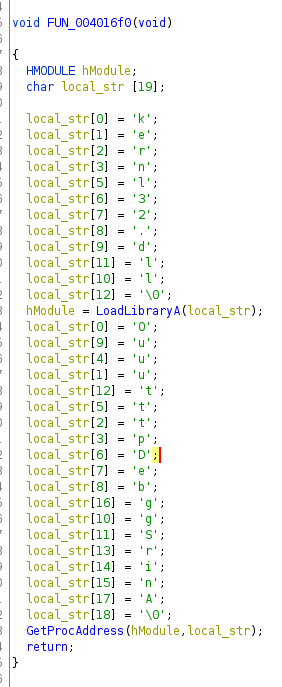
\includegraphics[scale=0.5]{immagini/load_library}
\caption{Risultato della de-compilazione dopo aver risolto il disassembling della \texttt{FUN\_004016f0}}
\label{Fig1}
\end{figure}

\begin{figure}
	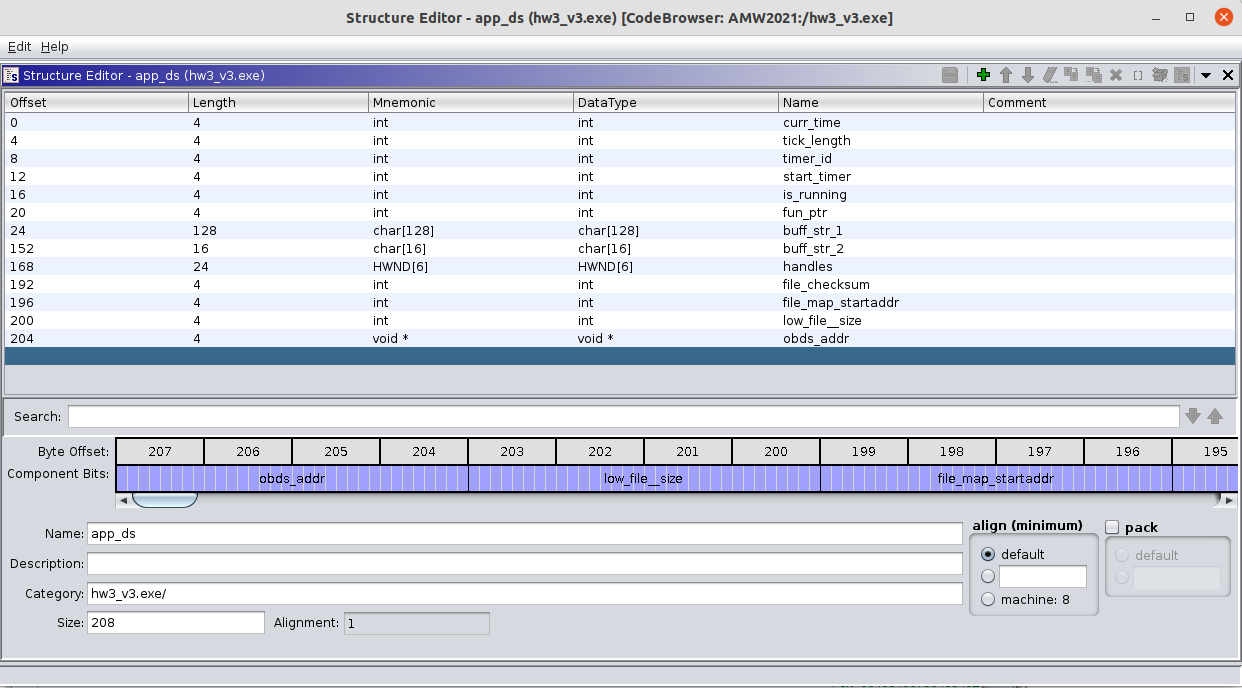
\includegraphics[scale=0.3]{immagini/hw3_struct.png}
	\caption{Struttura dati per il file hw3.exe}
	\label{Fig2}
\end{figure}

\vspace{10cm}

\begin{figure}[!h]
\begin{subfigure}{0.5\textwidth}
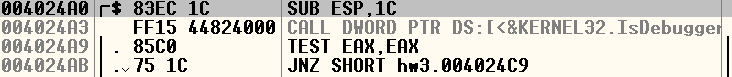
\includegraphics[scale=0.3]{immagini/odbg_1_before}
\end{subfigure}
\begin{subfigure}{0.5\textwidth}
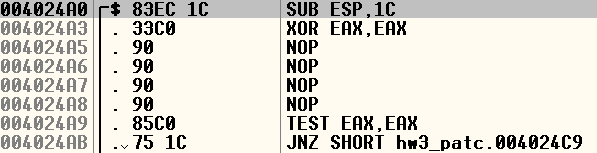
\includegraphics[scale=0.3]{immagini/odbg_1_after}
\end{subfigure}
\caption{Patch della funzione \texttt{IsDebuggerPresent}}
\label{Fig3}
\end{figure}

\begin{figure}[!h]
\begin{subfigure}{0.5\textwidth}
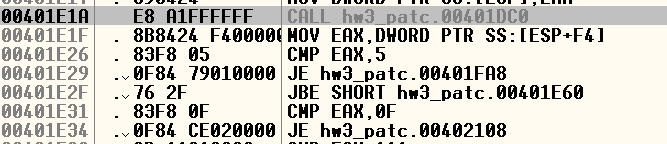
\includegraphics[scale=0.3]{immagini/odbg_2_before}
\end{subfigure}
\begin{subfigure}{0.5\textwidth}
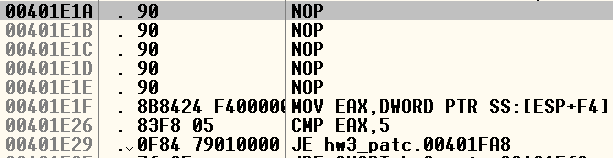
\includegraphics[scale=0.3]{immagini/odbg_2_after}
\end{subfigure}
\caption{Patch del campo \texttt{BeingDebugged} acceduto dalla PEB}
\label{Fig4}
\end{figure}

\begin{figure}[!h]
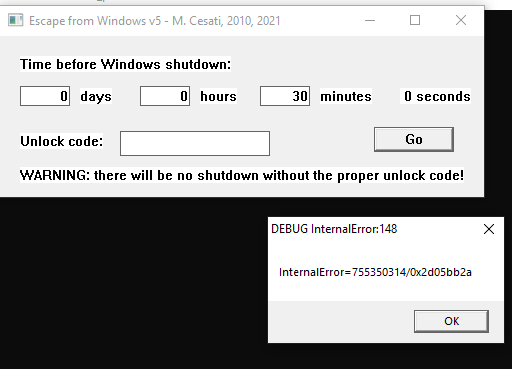
\includegraphics[scale=0.5]{immagini/internal_error}
\caption{Message Box dell' "Internal Error"}
\label{Fig5}
\end{figure}

\begin{figure}[!h]
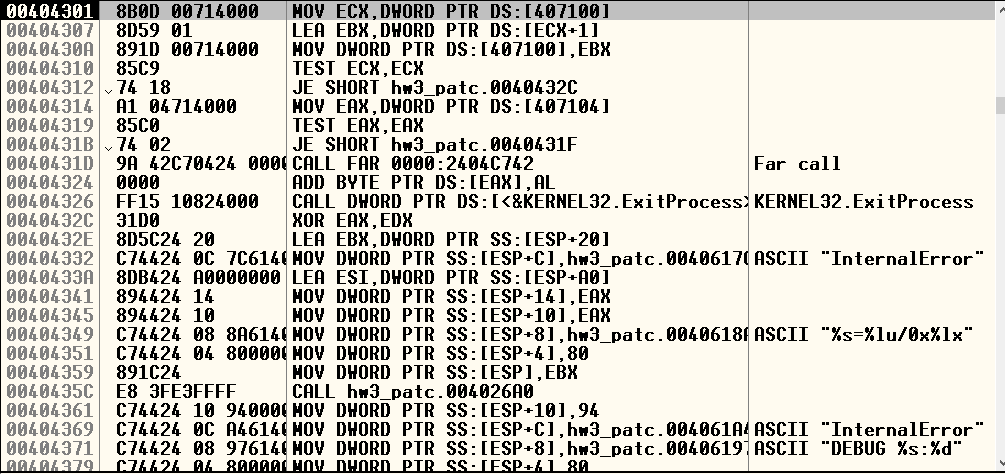
\includegraphics[scale=0.5]{immagini/internal_error_hint}
\caption{Stringhe relative al messaggio di "Internal Error"}
\label{Fig6}
\end{figure}

\vspace{10cm}

\begin{figure}
\begin{subfigure}{0.5\textwidth}
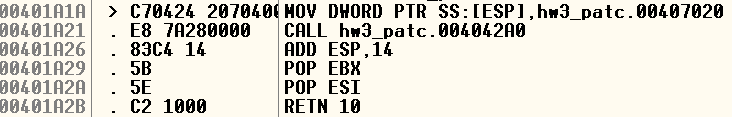
\includegraphics[scale=0.3]{immagini/odbg_3_before}
\end{subfigure}
\begin{subfigure}{0.5\textwidth}
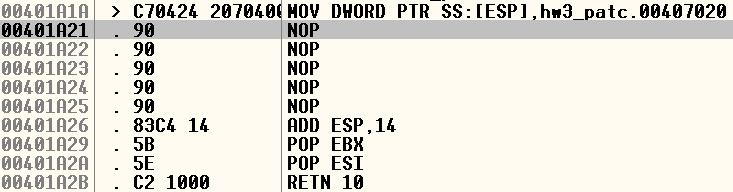
\includegraphics[scale=0.3]{immagini/odbg_3_after}
\end{subfigure}
\caption{Patch per la Message Box "Internal Error"}
\label{Fig7}
\end{figure}

\newpage
\begin{figure}
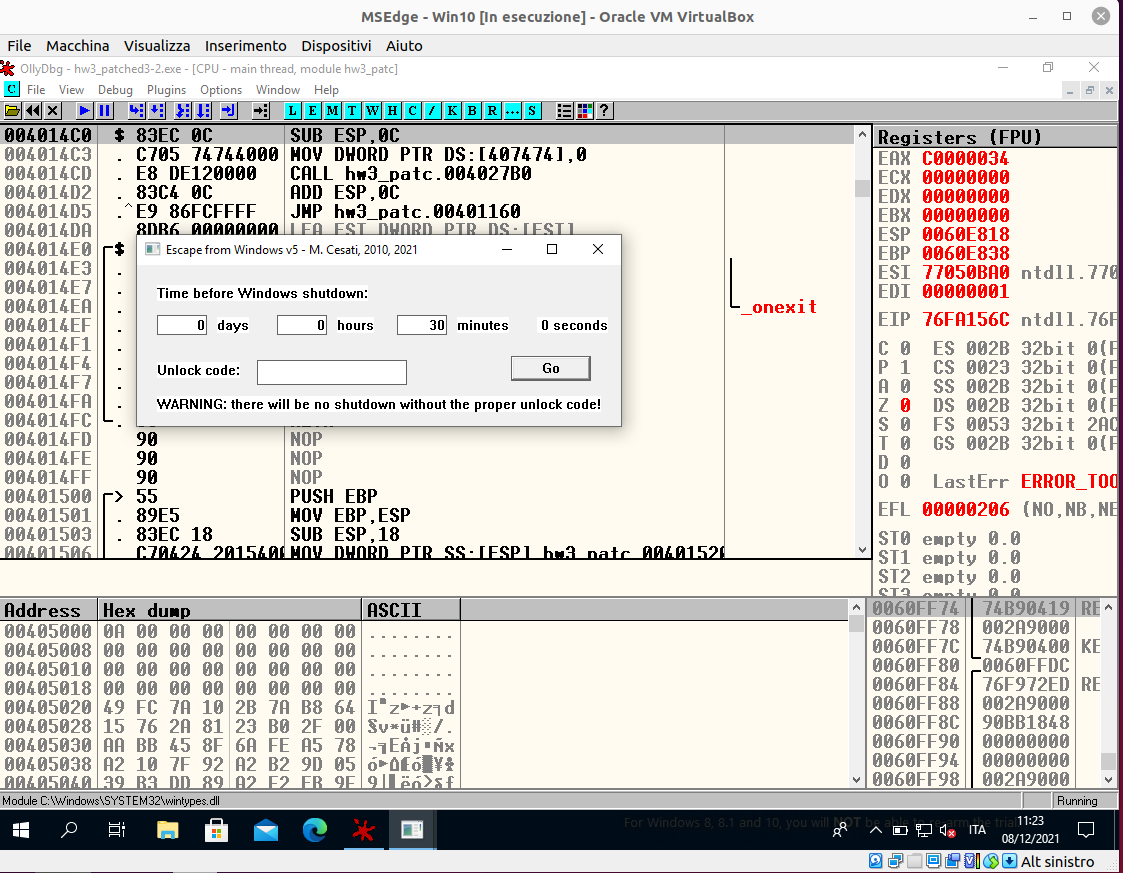
\includegraphics[scale=0.4]{immagini/correct_window_odbg}
\caption{Finestra correttamente mostrata nel debugger}
\label{Fig8}
\end{figure}
\end{document}





